\documentclass{standalone}
\usepackage{tikz}
\usetikzlibrary{shapes}
\usepackage{tikzpeople}

\begin{document}
				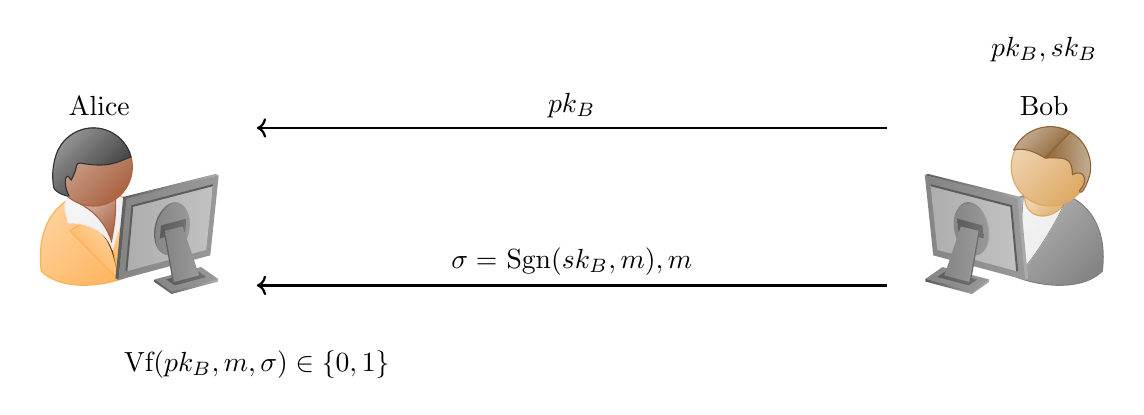
\begin{tikzpicture}
					\node[alice, monitor, label=Alice, minimum size=1.5cm] (Alice) at (0,0) {};
					\node[bob, mirrored, monitor, label=Bob, minimum size=1.5cm] (Bob) at (12,0) {};
					\node[] (pkGen) at (12,2) {${pk_B},{sk_B}$};
					\draw[<-, thick] (2,1)  -- (10,1) node[midway, above] {${pk_B}$};
					\draw[<-, thick] (2,-1)  -- (10,-1) node[midway, above] {$\sigma =$ Sgn$(sk_{B}, m),m$};
                    \node[] (dec) at (2,-2) {{Vf$(pk_B, m, \sigma) \in \{0,1\}$}};
					
				\end{tikzpicture}~\qquad\qquad
				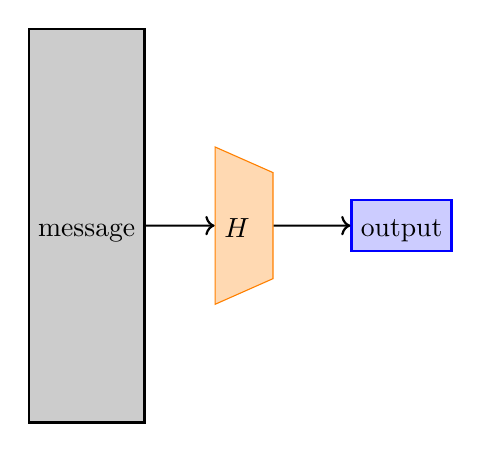
\begin{tikzpicture}
					\tikzstyle{RECT} = [thick, minimum width=1.25cm, minimum height=0.65cm, text height=2ex, text depth=0.25ex]
					\tikzstyle{TALL} = [thick, minimum width=1.25cm, minimum height =5cm, text height=2ex, text depth=0.25ex]
					\tikzstyle{output} = [RECT, draw=blue, fill=blue!20]
					\tikzstyle{message} = [TALL, draw=black, fill=black!20]
					\tikzstyle{HASH} = [trapezium, minimum width=2cm, text width=0.5cm, shape border rotate=270, text height=2ex, draw=orange, fill=orange!30, trapezium stretches=true, trapezium left angle=80, trapezium right angle=80]
					
					\node[message] (MSG) at (0,0) {message};
					\node[HASH] (HASH) at (2,0) {$H$};
					\draw[->,thick] (MSG.east) -- (HASH.west);
					\node[output] (OUT) at (4,0) {output};
					\draw[->,thick] (HASH.east) -- (OUT.west);
					%\draw [decorate,decoration={brace,amplitude=10pt},xshift=-4pt,yshift=0pt]
					%(-1,-2.5) -- (-1,2.5) node [black,midway,xshift=-1.25cm] 
					%{\footnotesize A lot of bits};
					%\draw [decorate,decoration={brace,amplitude=10pt},xshift=-4pt,yshift=0pt]
					%(5,0.5) -- (5,-0.5) node [black,midway,xshift=0.75cm] 
					%{\footnotesize $N$ bits};
				\end{tikzpicture}~\qquad~\qquad







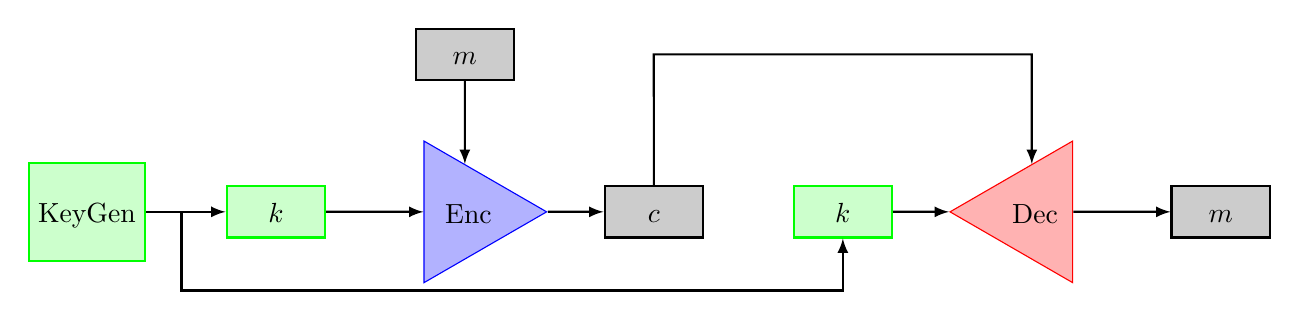
\begin{tikzpicture}[yscale=-1,xscale=0.8,>=latex]
				\tikzstyle{keys} = [thick, minimum width=1.25cm, minimum height=0.65cm, text height=2ex, text depth=0.25ex]
				\tikzstyle{key} = [keys, draw=green, fill=green!20]
				\tikzstyle{msg} = [keys, draw=black, fill=black!20]
				\tikzstyle{ctxt} = [keys, draw=black, fill=black!20]
				\tikzstyle{SQUA} = [thick, minimum width=1.25cm, minimum height =1.25cm, text height=2ex, text depth=0.25ex]
				\tikzstyle{GEN} = [SQUA, draw=green, fill=green!20]
				\tikzset{triangle/.style={draw,	shape border rotate=180,regular polygon,regular polygon sides=3, minimum height=0.65cm}}
				\tikzstyle{ENC} = [triangle, text width=0.5cm, shape border rotate=270, text height=2ex, draw=blue, fill=blue!30]
				\tikzstyle{DEC} = [triangle, text width=0.5cm, shape border rotate=90, text height=2ex, draw=red, fill=red!30]
				
				\node[GEN] (Gen) at (-3, 0) {KeyGen};
				\node[key] (EncKey) at (0,0) {$k$};
				\node[msg] (ptxt) at (3, -2) {$m$};
				\node[ENC] (Enc) at (3,0) {Enc};
				\node[ctxt] (ctxt) at (6,0) {$c$};
				\draw[->, thick] (Gen.east) -- (EncKey.west);
				\draw[->, thick] (EncKey.east) -- (Enc.west);
				\draw[->, thick] (ptxt.south) -- (Enc.north);
				\draw[->, thick] (Enc.east) -- (ctxt.west);
				
				\node[key] (DecKey) at (9,0) {$k$};
				\node[DEC] (Dec) at (12,0) {Dec};
				\node[ctxt] (ptxt) at (15,0) {$m$};
				\draw[->, thick] (Gen.east) -- (-1.5,0) -- (-1.5,1) -| (DecKey.south);
				\draw[->, thick] (DecKey.east) -- (Dec.west);
				\draw[->, thick] (Dec.east) -- (ptxt.west);
				\draw[->,thick] (ctxt.north) -- (6,-2) -| (Dec.north);
\end{tikzpicture}

\end{document}
